% Options for packages loaded elsewhere
\PassOptionsToPackage{unicode}{hyperref}
\PassOptionsToPackage{hyphens}{url}
%
\documentclass[
  a4paper,
]{article}
\usepackage{amsmath,amssymb}
\usepackage{iftex}
\ifPDFTeX
  \usepackage[T1]{fontenc}
  \usepackage[utf8]{inputenc}
  \usepackage{textcomp} % provide euro and other symbols
\else % if luatex or xetex
  \usepackage{unicode-math} % this also loads fontspec
  \defaultfontfeatures{Scale=MatchLowercase}
  \defaultfontfeatures[\rmfamily]{Ligatures=TeX,Scale=1}
\fi
\usepackage{lmodern}
\ifPDFTeX\else
  % xetex/luatex font selection
    \setmainfont[]{Helvetica}
\fi
% Use upquote if available, for straight quotes in verbatim environments
\IfFileExists{upquote.sty}{\usepackage{upquote}}{}
\IfFileExists{microtype.sty}{% use microtype if available
  \usepackage[]{microtype}
  \UseMicrotypeSet[protrusion]{basicmath} % disable protrusion for tt fonts
}{}
\makeatletter
\@ifundefined{KOMAClassName}{% if non-KOMA class
  \IfFileExists{parskip.sty}{%
    \usepackage{parskip}
  }{% else
    \setlength{\parindent}{0pt}
    \setlength{\parskip}{6pt plus 2pt minus 1pt}}
}{% if KOMA class
  \KOMAoptions{parskip=half}}
\makeatother
\usepackage{xcolor}
\usepackage[margin=0.75in]{geometry}
\usepackage{graphicx}
\makeatletter
\newsavebox\pandoc@box
\newcommand*\pandocbounded[1]{% scales image to fit in text height/width
  \sbox\pandoc@box{#1}%
  \Gscale@div\@tempa{\textheight}{\dimexpr\ht\pandoc@box+\dp\pandoc@box\relax}%
  \Gscale@div\@tempb{\linewidth}{\wd\pandoc@box}%
  \ifdim\@tempb\p@<\@tempa\p@\let\@tempa\@tempb\fi% select the smaller of both
  \ifdim\@tempa\p@<\p@\scalebox{\@tempa}{\usebox\pandoc@box}%
  \else\usebox{\pandoc@box}%
  \fi%
}
% Set default figure placement to htbp
\def\fps@figure{htbp}
\makeatother
\setlength{\emergencystretch}{3em} % prevent overfull lines
\providecommand{\tightlist}{%
  \setlength{\itemsep}{0pt}\setlength{\parskip}{0pt}}
\setcounter{secnumdepth}{-\maxdimen} % remove section numbering
\usepackage{titling}
\pretitle{\begin{flushleft}}
\posttitle{\end{flushleft}}
\usepackage{booktabs}
\usepackage{longtable}
\usepackage{float}
\floatplacement{figure}{H}
\usepackage{colortbl}
\usepackage{pdflscape}
\usepackage{tabu}
\usepackage{makecell}
\usepackage{xcolor}
\usepackage{soul}
\usepackage{caption}
\usepackage[singlelinecheck=false]{caption}
\usepackage[font={small,bf}]{caption}
\usepackage{multirow}
\usepackage{array}
\usepackage{lscape}
\newcommand{\blandscape}{\begin{landscape}}
\newcommand{\elandscape}{\end{landscape}}
\usepackage[dvipsnames]{xcolor}
\renewcommand{\footnotesize}{\tiny}
\usepackage{threeparttable}
\usepackage{booktabs}
\usepackage{longtable}
\usepackage{array}
\usepackage{multirow}
\usepackage{wrapfig}
\usepackage{float}
\usepackage{colortbl}
\usepackage{pdflscape}
\usepackage{tabu}
\usepackage{threeparttable}
\usepackage{threeparttablex}
\usepackage[normalem]{ulem}
\usepackage{makecell}
\usepackage{xcolor}
\usepackage{bookmark}
\IfFileExists{xurl.sty}{\usepackage{xurl}}{} % add URL line breaks if available
\urlstyle{same}
\hypersetup{
  hidelinks,
  pdfcreator={LaTeX via pandoc}}

\title{\vspace{-1.5cm} \begin{LARGE} WGS Quality Control Report \end{LARGE}}
\author{}
\date{\vspace{-2.5em}}

\begin{document}
\maketitle

\normalsize Batch Name: 2025-06-18\_P

\normalsize Experiment Name: 25ARS\_GHRUKPN\_Rpt\_LY9D3

\fontsize{7}{8}
\selectfont
\captionsetup[table]{labelformat=empty}
\renewcommand{\arraystretch}{1.2}

\begin{longtable}[t]{>{\centering\arraybackslash}p{1cm}>{\centering\arraybackslash}p{2.8cm}>{\centering\arraybackslash}p{1.5cm}>{\centering\arraybackslash}p{5cm}>{\centering\arraybackslash}p{5cm}}
\toprule
\multicolumn{1}{>{\centering\arraybackslash}p{1cm}}{\cellcolor[HTML]{D4D4D4}{\textbf{Isolate No.}}} & \multicolumn{1}{>{\centering\arraybackslash}p{2.8cm}}{\cellcolor[HTML]{D4D4D4}{\textbf{Sample ID}}} & \multicolumn{1}{>{\centering\arraybackslash}p{1.5cm}}{\cellcolor[HTML]{D4D4D4}{\textbf{Description}}} & \multicolumn{1}{>{\centering\arraybackslash}p{5cm}}{\cellcolor[HTML]{D4D4D4}{\textbf{ARSRL}}} & \multicolumn{1}{>{\centering\arraybackslash}p{5cm}}{\cellcolor[HTML]{D4D4D4}{\textbf{WGS}}}\\
\midrule
1 & 24ARS\_CRH0209 & 1396 & \em{Klebsiella pneumoniae} & \em{Klebsiella pneumoniae}\\
2 & 24ARS\_CVM0194 & 1397 & \em{Klebsiella pneumoniae} & \em{Klebsiella pneumoniae}\\
3 & 25ARS\_BGH0040 & 1228 & \em{Klebsiella pneumoniae} & \em{Klebsiella pneumoniae}\\
4 & 25ARS\_BGH0056 & 1236 & \em{Klebsiella pneumoniae} & \em{Klebsiella pneumoniae}\\
5 & 24ARS\_DMC0488 & 1399 & \em{Klebsiella pneumoniae} & \em{Klebsiella pneumoniae}\\
\addlinespace
6 & 25ARS\_CMC0016 & 1231 & \em{Klebsiella pneumoniae} & \em{Klebsiella pneumoniae}\\
7 & 25ARS\_DMC0033 & 1390 & \em{Klebsiella pneumoniae} & \em{Klebsiella pneumoniae}\\
8 & 25ARS\_DMC0034 & 1391 & \em{Klebsiella pneumoniae} & \em{Klebsiella pneumoniae}\\
9 & 25ARS\_BRH0009 & 1232 & \em{Klebsiella pneumoniae} & \em{Klebsiella pneumoniae}\\
10 & 25ARS\_JLM0007 & 1394 & \em{Klebsiella pneumoniae} & \em{Klebsiella pneumoniae}\\
\addlinespace
11 & 25ARS\_JLM0016 & 1242 & \em{Klebsiella pneumoniae} & \em{Klebsiella pneumoniae}\\
12 & 25ARS\_MAR0023 & 1240 & \em{Klebsiella pneumoniae} & \em{Klebsiella pneumoniae}\\
13 & 25ARS\_DMC0035 & 1392 & \em{Klebsiella pneumoniae} & \em{Klebsiella pneumoniae}\\
14 & 25ARS\_VSM0020 & 1222 & \em{Klebsiella pneumoniae} & \em{Klebsiella pneumoniae}\\
15 & 25ARS\_VSM0021 & 1223 & \em{Klebsiella pneumoniae} & \em{Klebsiella pneumoniae}\\
\addlinespace
16 & 25ARS\_NKI0007 & 1221 & \em{Klebsiella pneumoniae} & \em{Klebsiella quasipneumoniae}\\
17 & 24ARS\_JLM0249 & 1404 & \em{Klebsiella pneumoniae} & \em{Klebsiella quasipneumoniae}\\
\bottomrule
\multicolumn{5}{l}{\rule{0pt}{1em}\textit{Legend:} PASS   |   \colorbox{Salmon}{FAILURE}   |   \textcolor{Blue}{EXCEEDS THRESHOLD METRIC/S}   |   (x) - NON-CONCORDANT   |}\\
\end{longtable}

\fontsize{7}{8}
\selectfont
\captionsetup[table]{labelformat=empty}
\renewcommand{\arraystretch}{1.2}

\(\\\) \newpage

\begin{landscape}
\fontsize{7}{8}
\selectfont
\captionsetup[table]{labelformat=empty}
\renewcommand{\arraystretch}{1.2}

\begin{table}[!h]
\centering
\resizebox{\ifdim\width>\linewidth\linewidth\else\width\fi}{!}{
\begin{tabular}{cc>{}ccccccccc}
\toprule
\cellcolor[HTML]{D4D4D4}{\textbf{Isolate No.}} & \cellcolor[HTML]{D4D4D4}{\textbf{Sample ID}} & \cellcolor[HTML]{D4D4D4}{\textbf{WGS ID}} & \cellcolor[HTML]{D4D4D4}{\textbf{completeness}} & \cellcolor[HTML]{D4D4D4}{\textbf{contamination}} & \cellcolor[HTML]{D4D4D4}{\textbf{Depth of coverage}} & \cellcolor[HTML]{D4D4D4}{\textbf{Genome size}} & \cellcolor[HTML]{D4D4D4}{\textbf{GC content}} & \cellcolor[HTML]{D4D4D4}{\textbf{Contig count}} & \cellcolor[HTML]{D4D4D4}{\textbf{N50}} & \cellcolor[HTML]{D4D4D4}{\textbf{Mean read Q-score}}\\
\midrule
1 & 24ARS\_CRH0209 & \em{Klebsiella pneumoniae} & 100 & 1.1 & 59.4 & 5.52 Mb & 57 & 99 & 263765 & 35.5\\
2 & 24ARS\_CVM0194 & \em{Klebsiella pneumoniae} & 100 & 0.15 & 76.9 & 5.54 Mb & 57 & 85 & 203003 & 36.0\\
3 & 25ARS\_BGH0040 & \em{Klebsiella pneumoniae} & 100 & 0.62 & 69.9 & 5.66 Mb & 57 & 84 & 245672 & 35.6\\
4 & 25ARS\_BGH0056 & \em{Klebsiella pneumoniae} & 100 & 0.14 & 99.7 & 5.57 Mb & 57 & 93 & 189216 & 35.8\\
5 & 24ARS\_DMC0488 & \em{Klebsiella pneumoniae} & 100 & 0.11 & 62.9 & 5.57 Mb & 57 & 65 & 264952 & 35.5\\
\addlinespace
6 & 25ARS\_CMC0016 & \em{Klebsiella pneumoniae} & 100 & 0.07 & 56.6 & 5.51 Mb & 57 & 95 & 171026 & 35.5\\
7 & 25ARS\_DMC0033 & \em{Klebsiella pneumoniae} & 100 & 0.31 & 79.8 & 5.70 Mb & 57 & 130 & 233523 & 35.5\\
8 & 25ARS\_DMC0034 & \em{Klebsiella pneumoniae} & 100 & 0.07 & 59.1 & 5.56 Mb & 57 & 101 & 166266 & 35.7\\
9 & 25ARS\_BRH0009 & \em{Klebsiella pneumoniae} & 100 & 0.07 & 57.9 & 5.42 Mb & 57 & 91 & 247949 & 35.6\\
10 & 25ARS\_JLM0007 & \em{Klebsiella pneumoniae} & 100 & 0.88 & 67.2 & 5.65 Mb & 57 & 71 & 266766 & 35.0\\
\addlinespace
11 & 25ARS\_JLM0016 & \em{Klebsiella pneumoniae} & 100 & 0.07 & 87.2 & 5.47 Mb & 57 & 95 & 168723 & 35.2\\
12 & 25ARS\_MAR0023 & \em{Klebsiella pneumoniae} & 100 & 0.57 & 81.0 & 5.77 Mb & 57 & 89 & 342350 & 35.1\\
13 & 25ARS\_DMC0035 & \em{Klebsiella pneumoniae} & 100 & 0.21 & 68.3 & 5.21 Mb & 58 & 52 & 354837 & 35.4\\
14 & 25ARS\_VSM0020 & \em{Klebsiella pneumoniae} & 100 & 0.13 & 92.2 & 5.56 Mb & 57 & 71 & 295116 & 35.1\\
15 & 25ARS\_VSM0021 & \em{Klebsiella pneumoniae} & 100 & 0.54 & 99.0 & 5.72 Mb & 57 & 59 & 295875 & 36.0\\
\addlinespace
16 & 25ARS\_NKI0007 & \em{Klebsiella quasipneumoniae} & 100 & 0.15 & 60.5 & 5.60 Mb & 57 & 87 & 368309 & 35.2\\
17 & 24ARS\_JLM0249 & \em{Klebsiella quasipneumoniae} & 100 & 0.2 & 40.8 & 5.83 Mb & 57 & 165 & 83950 & 35.6\\
\bottomrule
\multicolumn{11}{l}{\rule{0pt}{1em}\textit{Legend:} PASS   |   \colorbox{Salmon}{FAILURE}   |   \textcolor{Blue}{EXCEEDS THRESHOLD METRIC/S}   |   (x) - NON-CONCORDANT   |}\\
\end{tabular}}
\end{table}









$\\$ $\\$ $\\$ $\color{red}{\normalsize\textbf{RECOMMENDATION:}}$



\begin{tabular}{>{\raggedright\arraybackslash}p{6cm}>{\centering\arraybackslash}p{6cm}>{\centering\arraybackslash}p{4cm}}
\toprule
\cellcolor[HTML]{D4D4D4}{\textbf{Sample ID}} & \cellcolor[HTML]{D4D4D4}{\textbf{Reason - Failed Metrics}} & \cellcolor[HTML]{D4D4D4}{\textbf{Remarks}}\\
\midrule
\cellcolor{gray!10}{} & \cellcolor{gray!10}{No further action required for this batch.} & \cellcolor{gray!10}{}\\
\bottomrule
\end{tabular}



\end{landscape}

\fontsize{7}{8}
\selectfont
\captionsetup[table]{labelformat=empty}
\renewcommand{\arraystretch}{1.2}

\begin{longtable}[l]{>{\raggedright\arraybackslash}p{8cm}c}
\toprule
\cellcolor[HTML]{D4D4D4}{\textbf{WGS\_ID}} & \cellcolor[HTML]{D4D4D4}{\textbf{Number}}\\
\midrule
\em{Klebsiella pneumoniae} & 15\\
\em{Klebsiella quasipneumoniae} & 2\\
\bottomrule
\end{longtable}

\begin{itemize}
\item
  \(\color{red}2\) distinct species were identified among
  \(\color{red}17\) isolates.
\item
  \(\color{red}100.00\) \% (n=17) of the isolates passed the QC, while
  \(\color{red}0.00\) \% (n=0) were tagged with failure.
\item
  Concordance between ARSRL and WGS species report was
  \(\color{red}100.00\) \%. \(\\\)
\end{itemize}

\subsubsection{GRAPHS}\label{graphs}

\fontsize{7}{8}
\selectfont
\captionsetup[table]{labelformat=empty}
\renewcommand{\arraystretch}{1.2}

\pandocbounded{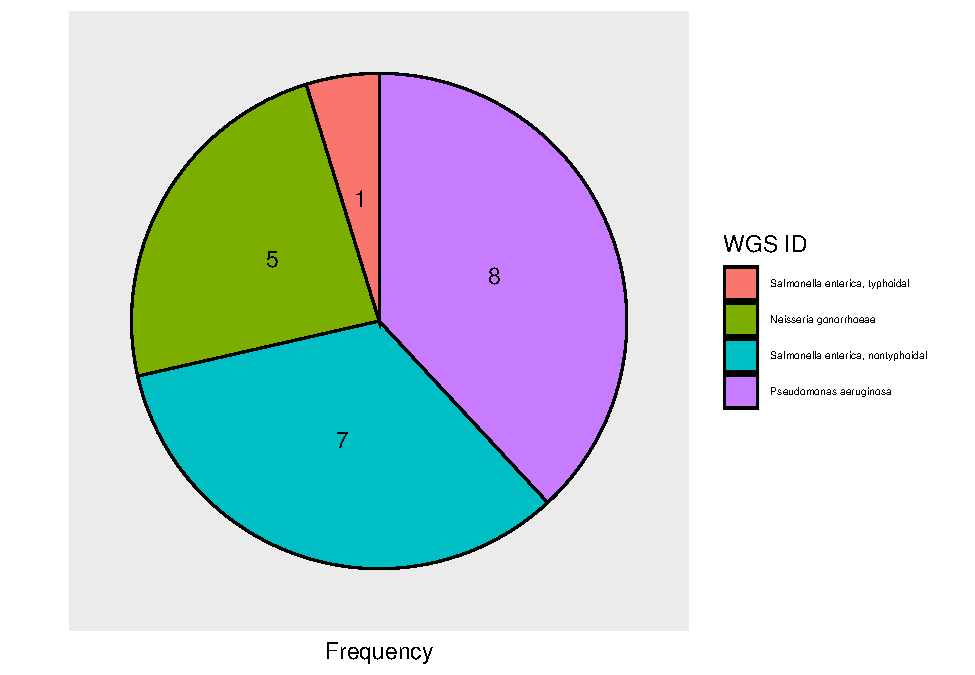
\includegraphics[keepaspectratio]{qualifyr_report_2025-06-18_P_files/figure-latex/pie_chart-1.pdf}}

\subsubsection{Result Classification}\label{result-classification}

\pandocbounded{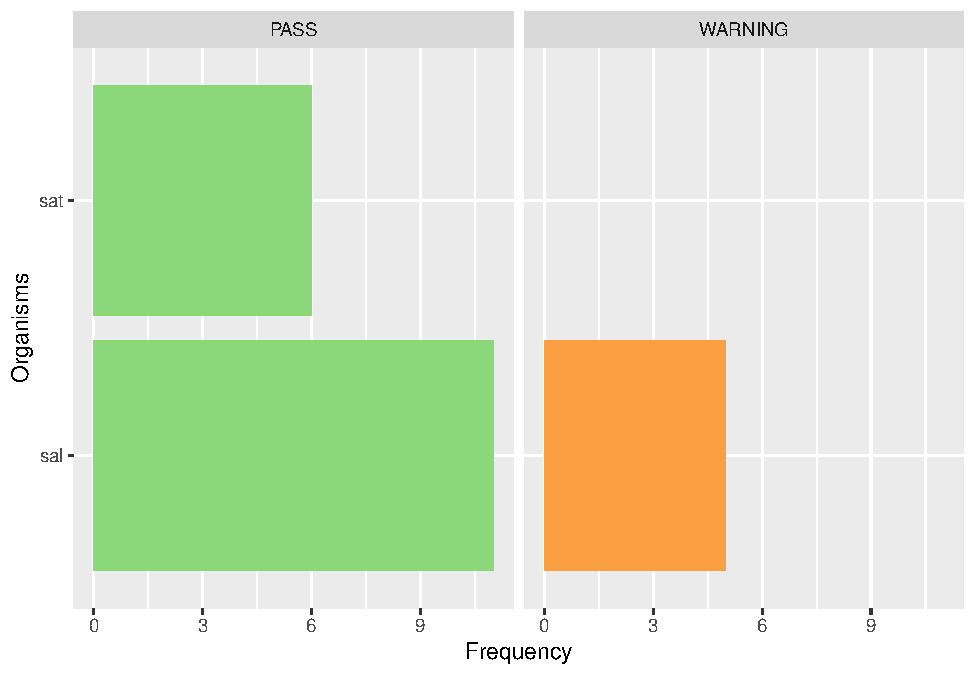
\includegraphics[keepaspectratio]{qualifyr_report_2025-06-18_P_files/figure-latex/organism results-1.pdf}}

\subsubsection{Number of contigs}\label{number-of-contigs}

\pandocbounded{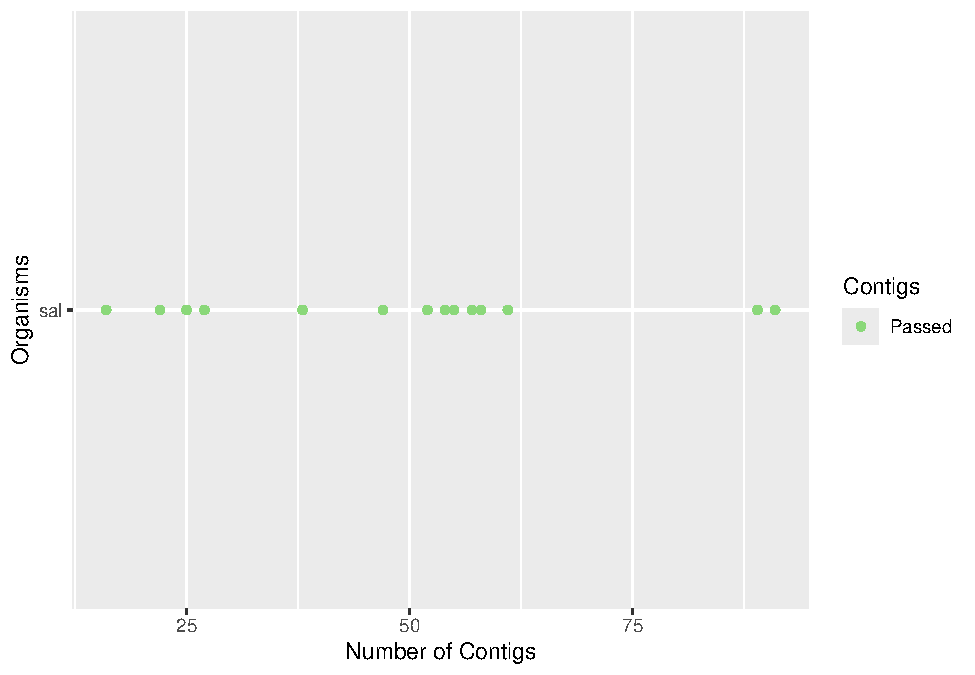
\includegraphics[keepaspectratio]{qualifyr_report_2025-06-18_P_files/figure-latex/unnamed-chunk-1-1.pdf}}

\subsubsection{N50 Value}\label{n50-value}

\pandocbounded{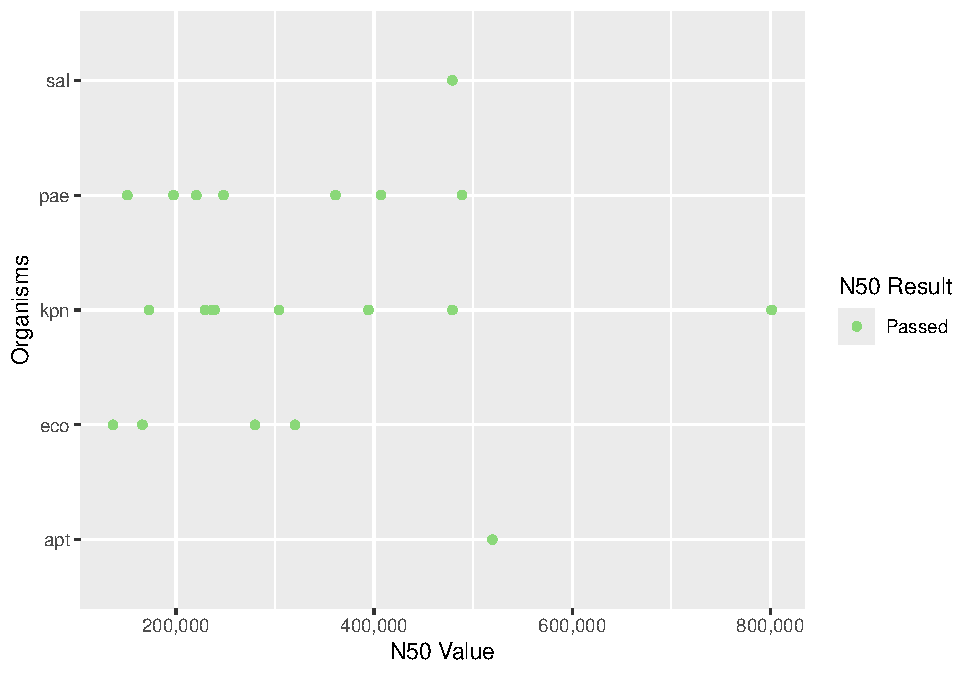
\includegraphics[keepaspectratio]{qualifyr_report_2025-06-18_P_files/figure-latex/n50_result -1.pdf}}

\subsubsection{Total Length}\label{total-length}

\pandocbounded{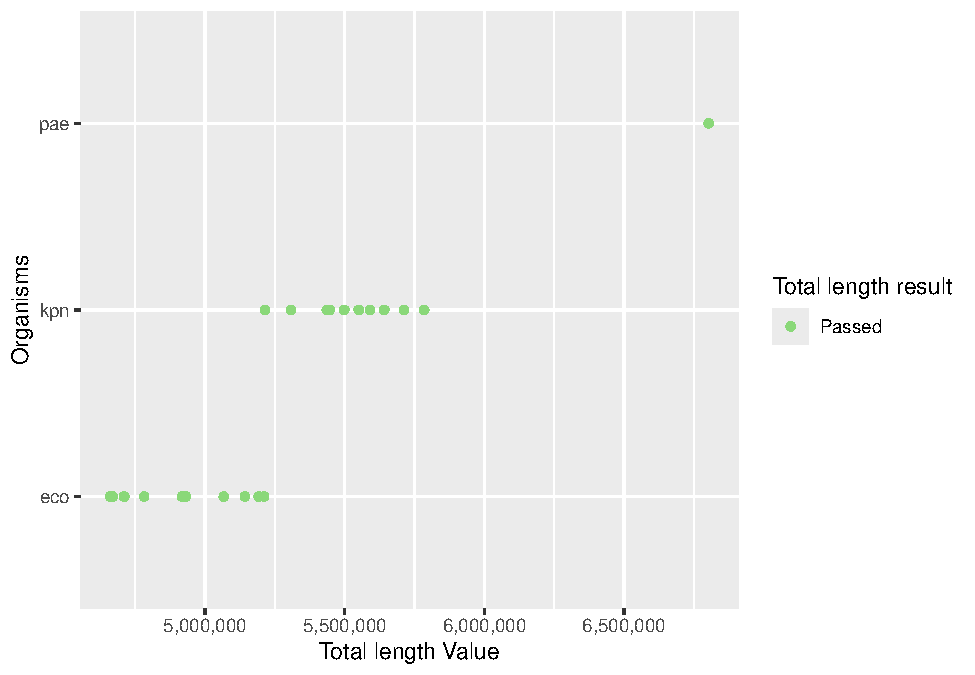
\includegraphics[keepaspectratio]{qualifyr_report_2025-06-18_P_files/figure-latex/length_result -1.pdf}}

\fontsize{7}{8}
\selectfont
\captionsetup[table]{labelformat=empty}
\renewcommand{\arraystretch}{1}

\subsubsection{MLST RESULTS}\label{mlst-results}

\begin{longtable}[l]{>{\centering\arraybackslash}p{3cm}>{\centering\arraybackslash}p{3cm}>{\centering\arraybackslash}p{1cm}>{\centering\arraybackslash}p{1cm}>{\centering\arraybackslash}p{1cm}>{\centering\arraybackslash}p{1cm}>{\centering\arraybackslash}p{1cm}>{\centering\arraybackslash}p{1cm}>{\centering\arraybackslash}p{1cm}>{\centering\arraybackslash}p{1cm}}
\toprule
\cellcolor[HTML]{D4D4D4}{\textbf{sample\_id}} & \cellcolor[HTML]{D4D4D4}{\textbf{species}} & \cellcolor[HTML]{D4D4D4}{\textbf{MLST}} & \cellcolor[HTML]{D4D4D4}{\textbf{gapA}} & \cellcolor[HTML]{D4D4D4}{\textbf{infB}} & \cellcolor[HTML]{D4D4D4}{\textbf{mdh}} & \cellcolor[HTML]{D4D4D4}{\textbf{pgi}} & \cellcolor[HTML]{D4D4D4}{\textbf{phoE}} & \cellcolor[HTML]{D4D4D4}{\textbf{rpoB}} & \cellcolor[HTML]{D4D4D4}{\textbf{tonB}}\\
\midrule
24ARS\_CRH0209 & \em{Klebsiella pneumoniae} & - & 2 & \textasciitilde{}245 & 11 & 1 & 9 & 4 & 242\\
24ARS\_CVM0194 & \em{Klebsiella pneumoniae} & 11 & 3 & 3 & 1 & 1 & 1 & 1 & 4\\
24ARS\_DMC0488 & \em{Klebsiella pneumoniae} & 101 & 2 & 6 & 1 & 5 & 4 & 1 & 6\\
24ARS\_JLM0249 & \em{Klebsiella quasipneumoniae} & 571 & 17 & 19 & 79 & 20 & 108 & 55 & 142\\
25ARS\_BGH0040 & \em{Klebsiella pneumoniae} & 147 & 3 & 4 & 6 & 1 & 7 & 4 & 38\\
\addlinespace
25ARS\_BGH0056 & \em{Klebsiella pneumoniae} & 15 & 1 & 1 & 1 & 1 & 1 & 1 & 1\\
25ARS\_BRH0009 & \em{Klebsiella pneumoniae} & 29 & 2 & 3 & 2 & 2 & 6 & 4 & 4\\
25ARS\_CMC0016 & \em{Klebsiella pneumoniae} & 15 & 1 & 1 & 1 & 1 & 1 & 1 & 1\\
25ARS\_DMC0033 & \em{Klebsiella pneumoniae} & 219 & 2 & 1 & 2 & 3 & 27 & 1 & 39\\
25ARS\_DMC0034 & \em{Klebsiella pneumoniae} & 15 & 1 & 1 & 1 & 1 & 1 & 1 & 1\\
\addlinespace
25ARS\_DMC0035 & \em{Klebsiella pneumoniae} & 5616 & 3 & 4 & 6 & 5 & 7 & 4 & 38\\
25ARS\_JLM0007 & \em{Klebsiella pneumoniae} & 147 & 3 & 4 & 6 & 1 & 7 & 4 & 38\\
25ARS\_JLM0016 & \em{Klebsiella pneumoniae} & 11 & 3 & 3 & 1 & 1 & 1 & 1 & 4\\
25ARS\_MAR0023 & \em{Klebsiella pneumoniae} & 39 & 2 & 1 & 2 & 4 & 9 & 1 & 14\\
25ARS\_NKI0007 & \em{Klebsiella quasipneumoniae} & - & 42 & 15 & 18 & 372 & 11 & 13 & 51\\
\addlinespace
25ARS\_VSM0020 & \em{Klebsiella pneumoniae} & 17 & 2 & 1 & 1 & 1 & 4 & 4 & 4\\
25ARS\_VSM0021 & \em{Klebsiella pneumoniae} & 147 & 3 & 4 & 6 & 1 & 7 & 4 & 38\\
\bottomrule
\multicolumn{10}{l}{\rule{0pt}{1em}\textit{Legend: } (-) Not identified}\\
\end{longtable}

\subsubsection{MLST RESULTS SUMMARY:}\label{mlst-results-summary}

\begin{longtable}[l]{>{\raggedright\arraybackslash}p{6cm}>{\raggedright\arraybackslash}p{10cm}}
\toprule
\cellcolor[HTML]{D4D4D4}{\textbf{wgs\_id}} & \cellcolor[HTML]{D4D4D4}{\textbf{mlst\_count}}\\
\midrule
\em{Klebsiella pneumoniae} & - (n= 1 ), 11 (n= 2 ), 101 (n= 1 ), 147 (n= 3 ), 15 (n= 3 ), 29 (n= 1 ), 219 (n= 1 ), 5616 (n= 1 ), 39 (n= 1 ), 17 (n= 1 )\\
\em{Klebsiella quasipneumoniae} & - (n= 1 ), 571 (n= 1 )\\
\bottomrule
\multicolumn{2}{l}{\rule{0pt}{1em}\textit{Legend: } (-) Not identified}\\
\end{longtable}

\newpage
\begin{landscape}
\fontsize{7}{8}
\selectfont
\captionsetup[table]{labelformat=empty}
\renewcommand{\arraystretch}{1.2}


\normalsize\textbf{AMR PREDICTION RESULTS}\textbf\normalsize




\fontsize{7}{8}
\selectfont
\captionsetup[table]{labelformat=empty}
\renewcommand{\arraystretch}{1.2}

\begingroup\fontsize{7}{9}\selectfont

\resizebox{\ifdim\width>\linewidth\linewidth\else\width\fi}{!}{
\begin{tabular}{c>{\centering\arraybackslash}p{3cm}>{\centering\arraybackslash}p{3cm}>{\centering\arraybackslash}p{3cm}>{\centering\arraybackslash}p{3cm}>{\centering\arraybackslash}p{3cm}>{\centering\arraybackslash}p{3cm}}
\toprule
\multicolumn{7}{l}{\textbf{\textit{Klebsiella pneumoniae} (Part 1.1)}} \\
\cmidrule(l{3pt}r{3pt}){1-7}
\cellcolor[HTML]{D4D4D4}{\textbf{sample\_id}} & \cellcolor[HTML]{D4D4D4}{\textbf{AMR AMIKACIN/ KAMYCIN}} & \cellcolor[HTML]{D4D4D4}{\textbf{AMR AMIKACIN/ KAMYCIN/ QUINOLONE/ TOBRAMYCIN}} & \cellcolor[HTML]{D4D4D4}{\textbf{AMR AMIKACIN/ KAMYCIN/ TOBRAMYCIN}} & \cellcolor[HTML]{D4D4D4}{\textbf{AMR AMINOGLYCOSIDE}} & \cellcolor[HTML]{D4D4D4}{\textbf{AMR AZITHROMYCIN/ ERYTHROMYCIN/ SPIRAMYCIN/ TELITHROMYCIN}} & \cellcolor[HTML]{D4D4D4}{\textbf{AMR AZITHROMYCIN/ ERYTHROMYCIN/ STREPTOGRAMIN}}\\
\midrule
24ARS\_CRH0209 & NA & NA & NA & NA & mph(A) & NA\\
24ARS\_CVM0194 & NA & aac(6')-Ib-cr5 & NA & NA & mph(A) & msr(E)\\
24ARS\_DMC0488 & NA & aac(6')-Ib-cr5 & NA & rmtB1 & mph(A) & NA\\
24ARS\_JLM0249 & NA & aac(6')-Ib-cr5 & NA & NA & mph(A) & NA\\
25ARS\_BGH0040 & NA & aac(6')-Ib-cr5 & NA & NA & mph(A) & NA\\
\addlinespace
25ARS\_BGH0056 & NA & aac(6')-Ib-cr5 & NA & rmtB1 & mph(A) & NA\\
\bottomrule
\end{tabular}}
\endgroup{}


\vspace{5mm}

\begingroup\fontsize{7}{9}\selectfont

\resizebox{\ifdim\width>\linewidth\linewidth\else\width\fi}{!}{
\begin{tabular}{c>{\centering\arraybackslash}p{3cm}>{\centering\arraybackslash}p{3cm}>{\centering\arraybackslash}p{3cm}>{\centering\arraybackslash}p{3cm}>{\centering\arraybackslash}p{3cm}>{\centering\arraybackslash}p{3cm}}
\toprule
\multicolumn{7}{l}{\textbf{\textit{Klebsiella pneumoniae} (Part 1.2)}} \\
\cmidrule(l{3pt}r{3pt}){1-7}
\cellcolor[HTML]{D4D4D4}{\textbf{sample\_id}} & \cellcolor[HTML]{D4D4D4}{\textbf{AMR BETA-LACTAM}} & \cellcolor[HTML]{D4D4D4}{\textbf{AMR BLEOMYCIN}} & \cellcolor[HTML]{D4D4D4}{\textbf{AMR CARBAPENEM}} & \cellcolor[HTML]{D4D4D4}{\textbf{AMR CEPHALOSPORIN}} & \cellcolor[HTML]{D4D4D4}{\textbf{AMR CHLORAMPHENICOL}} & \cellcolor[HTML]{D4D4D4}{\textbf{AMR CHLORAMPHENICOL/ FLORFENICOL}}\\
\midrule
24ARS\_CRH0209 & blaSHV-11, blaTEM-1 & ble & blaNDM-5 & NA & NA & NA\\
24ARS\_CVM0194 & blaSHV-11, blaTEM-1, blaOXA & ble & blaNDM-7 & blaCTX-M-15 & catB3 & NA\\
24ARS\_DMC0488 & blaTEM, blaTEM, blaSHV-1 & ble & blaNDM-5 & blaCTX-M-15 & NA & NA\\
24ARS\_JLM0249 & blaOKP-A-17 & ble & blaNDM-5 & blaCTX-M-15, blaOXA-1 & catB3 & NA\\
25ARS\_BGH0040 & blaSHV-11 & ble & blaNDM-5 & blaCTX-M-15, blaOXA-1 & catB3 & NA\\
\addlinespace
25ARS\_BGH0056 & blaOXA, blaTEM-1, blaSHV-28 & ble & blaNDM-5 & blaCTX-M-15 & catB3 & NA\\
\bottomrule
\end{tabular}}
\endgroup{}


\vspace{5mm}

\begingroup\fontsize{7}{9}\selectfont

\resizebox{\ifdim\width>\linewidth\linewidth\else\width\fi}{!}{
\begin{tabular}{c>{\centering\arraybackslash}p{3cm}>{\centering\arraybackslash}p{3cm}>{\centering\arraybackslash}p{3cm}>{\centering\arraybackslash}p{3cm}>{\centering\arraybackslash}p{3cm}>{\centering\arraybackslash}p{3cm}}
\toprule
\multicolumn{7}{l}{\textbf{\textit{Klebsiella pneumoniae} (Part 1.3)}} \\
\cmidrule(l{3pt}r{3pt}){1-7}
\cellcolor[HTML]{D4D4D4}{\textbf{sample\_id}} & \cellcolor[HTML]{D4D4D4}{\textbf{AMR CLINDAMYCIN/ ERYTHROMYCIN}} & \cellcolor[HTML]{D4D4D4}{\textbf{AMR CLINDAMYCIN/ ERYTHROMYCIN/ STREPTOGRAMIN B}} & \cellcolor[HTML]{D4D4D4}{\textbf{AMR COLISTIN}} & \cellcolor[HTML]{D4D4D4}{\textbf{AMR EFFLUX}} & \cellcolor[HTML]{D4D4D4}{\textbf{AMR ERYTHROMYCIN}} & \cellcolor[HTML]{D4D4D4}{\textbf{AMR FOSFOMYCIN}}\\
\midrule
24ARS\_CRH0209 & NA & NA & NA & kdeA, emrD & NA & fosA\\
24ARS\_CVM0194 & erm(42) & NA & NA & kdeA, emrD & mph(E) & fosA\\
24ARS\_DMC0488 & NA & erm(B) & NA & emrD, kdeA & NA & fosA\\
24ARS\_JLM0249 & NA & NA & NA & emrD, kdeA & NA & fosA\\
25ARS\_BGH0040 & NA & NA & NA & emrD, kdeA & NA & fosA\\
\addlinespace
25ARS\_BGH0056 & NA & erm(B) & mcr-1.1 & emrD, kdeA & NA & fosA\\
\bottomrule
\end{tabular}}
\endgroup{}


\vspace{5mm}

\begingroup\fontsize{7}{9}\selectfont

\resizebox{\ifdim\width>\linewidth\linewidth\else\width\fi}{!}{
\begin{tabular}{c>{\centering\arraybackslash}p{3cm}>{\centering\arraybackslash}p{3cm}>{\centering\arraybackslash}p{3cm}>{\centering\arraybackslash}p{3cm}>{\centering\arraybackslash}p{3cm}>{\centering\arraybackslash}p{3cm}}
\toprule
\multicolumn{7}{l}{\textbf{\textit{Klebsiella pneumoniae} (Part 1.4)}} \\
\cmidrule(l{3pt}r{3pt}){1-7}
\cellcolor[HTML]{D4D4D4}{\textbf{sample\_id}} & \cellcolor[HTML]{D4D4D4}{\textbf{AMR GENTAMICIN}} & \cellcolor[HTML]{D4D4D4}{\textbf{AMR KAMYCIN}} & \cellcolor[HTML]{D4D4D4}{\textbf{AMR PHENICOL/ QUINOLONE}} & \cellcolor[HTML]{D4D4D4}{\textbf{AMR QUINOLONE}} & \cellcolor[HTML]{D4D4D4}{\textbf{AMR RIFAMYCIN}} & \cellcolor[HTML]{D4D4D4}{\textbf{AMR STREPTOMYCIN}}\\
\midrule
24ARS\_CRH0209 & NA & NA & oqxB20, oqxA & NA & NA & NA\\
24ARS\_CVM0194 & aac(3)-IIe & aph(3')-Ia & oqxB, oqxA & qnrS1 & NA & NA\\
24ARS\_DMC0488 & NA & NA & oqxA, oqxB20 & qnrB6 & arr-3 & aadA2\\
24ARS\_JLM0249 & NA & NA & oqxB, oqxA & qnrS1 & NA & aadA2, aph(3'')-Ib, aph(6)-Id\\
25ARS\_BGH0040 & NA & NA & oqxA, oqxB & qnrS1, qnrB6 & arr-3 & aph(3'')-Ib, aph(6)-Id, aadA16, aadA2\\
\addlinespace
25ARS\_BGH0056 & NA & NA & oqxB, oqxA & qnrB1 & NA & aadA2, aph(3'')-Ib, aph(6)-Id\\
\bottomrule
\end{tabular}}
\endgroup{}


\vspace{5mm}

\begingroup\fontsize{7}{9}\selectfont

\resizebox{\ifdim\width>\linewidth\linewidth\else\width\fi}{!}{
\begin{tabular}{c>{\centering\arraybackslash}p{3cm}>{\centering\arraybackslash}p{3cm}>{\centering\arraybackslash}p{3cm}>{\centering\arraybackslash}p{3cm}>{\centering\arraybackslash}p{3cm}>{\centering\arraybackslash}p{3cm}}
\toprule
\multicolumn{7}{l}{\textbf{\textit{Klebsiella pneumoniae} (Part 1.5)}} \\
\cmidrule(l{3pt}r{3pt}){1-7}
\cellcolor[HTML]{D4D4D4}{\textbf{sample\_id}} & \cellcolor[HTML]{D4D4D4}{\textbf{AMR SULFOMIDE}} & \cellcolor[HTML]{D4D4D4}{\textbf{AMR TETRACYCLINE}} & \cellcolor[HTML]{D4D4D4}{\textbf{AMR TRIMETHOPRIM}} & \cellcolor[HTML]{D4D4D4}{\textbf{STRESS }} & \cellcolor[HTML]{D4D4D4}{\textbf{STRESS ARSENIC}} & \cellcolor[HTML]{D4D4D4}{\textbf{STRESS ARSENITE}}\\
\midrule
24ARS\_CRH0209 & NA & tet(A) & NA & fieF, asr & arsR & arsB, arsA, arsD\\
24ARS\_CVM0194 & sul1 & NA & NA & asr, fieF, hsp20, clpK & arsR & arsB, arsD, arsA\\
24ARS\_DMC0488 & sul1 & NA & dfrA27, dfrA12 & fieF & NA & NA\\
24ARS\_JLM0249 & sul1, sul2 & NA & dfrA12 & asr, fieF & arsR & arsB, arsA, arsD\\
25ARS\_BGH0040 & sul2, sul1 & tet(D) & dfrA12, dfrA27 & fieF, hsp20, clpK & NA & NA\\
\addlinespace
25ARS\_BGH0056 & sul1, sul2 & tet(A) & dfrA14, dfrA12 & fieF, asr & NA & NA\\
\bottomrule
\end{tabular}}
\endgroup{}


\vspace{5mm}

\begingroup\fontsize{7}{9}\selectfont

\resizebox{\ifdim\width>\linewidth\linewidth\else\width\fi}{!}{
\begin{tabular}{c>{\centering\arraybackslash}p{3cm}>{\centering\arraybackslash}p{3cm}>{\centering\arraybackslash}p{3cm}>{\centering\arraybackslash}p{3cm}>{\centering\arraybackslash}p{3cm}>{\centering\arraybackslash}p{3cm}}
\toprule
\multicolumn{7}{l}{\textbf{\textit{Klebsiella pneumoniae} (Part 1.6)}} \\
\cmidrule(l{3pt}r{3pt}){1-7}
\cellcolor[HTML]{D4D4D4}{\textbf{sample\_id}} & \cellcolor[HTML]{D4D4D4}{\textbf{STRESS ARSETE}} & \cellcolor[HTML]{D4D4D4}{\textbf{STRESS COPPER}} & \cellcolor[HTML]{D4D4D4}{\textbf{STRESS COPPER/ SILVER}} & \cellcolor[HTML]{D4D4D4}{\textbf{STRESS MERCURY}} & \cellcolor[HTML]{D4D4D4}{\textbf{STRESS ORGANOMERCURY}} & \cellcolor[HTML]{D4D4D4}{\textbf{STRESS QUATERRY AMMONIUM}}\\
\midrule
24ARS\_CRH0209 & arsC, arsC & pcoC, pcoB, pcoS, pcoR, pcoD, pcoA & silA, silB, silF, silC, silR, silS & NA & NA & NA\\
24ARS\_CVM0194 & arsC, arsC & NA & silS, silR, silC, silF, silB, silA & NA & NA & NA\\
24ARS\_DMC0488 & arsC & NA & NA & NA & NA & qacEdelta1\\
24ARS\_JLM0249 & arsC, arsC, arsC & pcoD, pcoR, pcoA, pcoB, pcoC, pcoS & silS, silR, silC, silF, silB, silA & NA & NA & qacEdelta1\\
25ARS\_BGH0040 & arsC & pcoA, pcoB, pcoC, pcoD, pcoR, pcoS, pcoE & silS, silR, silC, silF, silB, silA & merE, merD, merA, merP, merT, merR & merC & qacEdelta1\\
\addlinespace
25ARS\_BGH0056 & arsC & pcoC, pcoB, pcoA, pcoS, pcoR, pcoD & silA, silB, silF, silC, silR, silS & merF, merA, merD, merR, merT, merP, merE & NA & qacEdelta1\\
\bottomrule
\end{tabular}}
\endgroup{}


\vspace{5mm}

\begingroup\fontsize{7}{9}\selectfont

\resizebox{\ifdim\width>\linewidth\linewidth\else\width\fi}{!}{
\begin{tabular}{c>{\centering\arraybackslash}p{3cm}>{\centering\arraybackslash}p{3cm}>{\centering\arraybackslash}p{3cm}}
\toprule
\multicolumn{4}{l}{\textbf{\textit{Klebsiella pneumoniae} (Part 1.7)}} \\
\cmidrule(l{3pt}r{3pt}){1-4}
\cellcolor[HTML]{D4D4D4}{\textbf{sample\_id}} & \cellcolor[HTML]{D4D4D4}{\textbf{STRESS SILVER}} & \cellcolor[HTML]{D4D4D4}{\textbf{STRESS TELLURIUM}} & \cellcolor[HTML]{D4D4D4}{\textbf{VIRULENCE }}\\
\midrule
24ARS\_CRH0209 & silP, silE & NA & NA\\
24ARS\_CVM0194 & silE, silP & NA & ybtP, ybtQ\\
24ARS\_DMC0488 & NA & NA & ybtQ, ybtP\\
24ARS\_JLM0249 & silE, silP & terE, terD, terC, terB & NA\\
25ARS\_BGH0040 & silE, silP & terE, terB, terC, terD & NA\\
\addlinespace
25ARS\_BGH0056 & silP, silE & NA & ybtP, ybtQ\\
\bottomrule
\end{tabular}}
\endgroup{}


\vspace{10mm}

\begingroup\fontsize{7}{9}\selectfont

\resizebox{\ifdim\width>\linewidth\linewidth\else\width\fi}{!}{
\begin{tabular}{l>{\centering\arraybackslash}p{3cm}>{\centering\arraybackslash}p{3cm}>{\centering\arraybackslash}p{3cm}>{\centering\arraybackslash}p{3cm}>{\centering\arraybackslash}p{3cm}>{\centering\arraybackslash}p{3cm}c}
\toprule
\multicolumn{7}{l}{\textbf{\textit{Klebsiella pneumoniae} (Part 2.1)}} \\
\cmidrule(l{3pt}r{3pt}){1-7}
\cellcolor[HTML]{D4D4D4}{\textbf{ }} & \cellcolor[HTML]{D4D4D4}{\textbf{sample\_id}} & \cellcolor[HTML]{D4D4D4}{\textbf{AMR AMIKACIN/ KAMYCIN}} & \cellcolor[HTML]{D4D4D4}{\textbf{AMR AMIKACIN/ KAMYCIN/ QUINOLONE/ TOBRAMYCIN}} & \cellcolor[HTML]{D4D4D4}{\textbf{AMR AMIKACIN/ KAMYCIN/ TOBRAMYCIN}} & \cellcolor[HTML]{D4D4D4}{\textbf{AMR AMINOGLYCOSIDE}} & \cellcolor[HTML]{D4D4D4}{\textbf{AMR AZITHROMYCIN/ ERYTHROMYCIN/ SPIRAMYCIN/ TELITHROMYCIN}} & \cellcolor[HTML]{D4D4D4}{\textbf{AMR AZITHROMYCIN/ ERYTHROMYCIN/ STREPTOGRAMIN}}\\
\midrule
7 & 25ARS\_BRH0009 & NA & NA & NA & rmtC & NA & NA\\
8 & 25ARS\_CMC0016 & NA & aac(6')-Ib-cr5 & NA & rmtC & mph(A) & NA\\
9 & 25ARS\_DMC0033 & aph(3')-VI & aac(6')-Ib-cr5 & NA & NA & mph(A) & NA\\
10 & 25ARS\_DMC0034 & NA & aac(6')-Ib-cr5 & NA & rmtC & mph(A) & NA\\
11 & 25ARS\_DMC0035 & NA & NA & NA & rmtB1 & mph(A) & NA\\
\addlinespace
12 & 25ARS\_JLM0007 & NA & NA & aac(6')-Ib & NA & mph(A) & NA\\
\bottomrule
\end{tabular}}
\endgroup{}


\vspace{5mm}

\begingroup\fontsize{7}{9}\selectfont

\resizebox{\ifdim\width>\linewidth\linewidth\else\width\fi}{!}{
\begin{tabular}{l>{\centering\arraybackslash}p{3cm}>{\centering\arraybackslash}p{3cm}>{\centering\arraybackslash}p{3cm}>{\centering\arraybackslash}p{3cm}>{\centering\arraybackslash}p{3cm}>{\centering\arraybackslash}p{3cm}c}
\toprule
\multicolumn{7}{l}{\textbf{\textit{Klebsiella pneumoniae} (Part 2.2)}} \\
\cmidrule(l{3pt}r{3pt}){1-7}
\cellcolor[HTML]{D4D4D4}{\textbf{ }} & \cellcolor[HTML]{D4D4D4}{\textbf{sample\_id}} & \cellcolor[HTML]{D4D4D4}{\textbf{AMR BETA-LACTAM}} & \cellcolor[HTML]{D4D4D4}{\textbf{AMR BLEOMYCIN}} & \cellcolor[HTML]{D4D4D4}{\textbf{AMR CARBAPENEM}} & \cellcolor[HTML]{D4D4D4}{\textbf{AMR CEPHALOSPORIN}} & \cellcolor[HTML]{D4D4D4}{\textbf{AMR CHLORAMPHENICOL}} & \cellcolor[HTML]{D4D4D4}{\textbf{AMR CHLORAMPHENICOL/ FLORFENICOL}}\\
\midrule
7 & 25ARS\_BRH0009 & blaTEM-1 & ble & blaNDM-1 & blaSHV-187, blaCTX-M-15 & NA & NA\\
8 & 25ARS\_CMC0016 & blaTEM-1, blaSHV-28 & ble & blaNDM-1 & blaCTX-M-15 & catA2 & NA\\
9 & 25ARS\_DMC0033 & blaTEM, blaSHV-1, blaOXA-9 & ble & blaNDM-1 & blaCTX-M-15 & NA & NA\\
10 & 25ARS\_DMC0034 & blaTEM-1, blaSHV-28 & ble & blaNDM-1 & blaCTX-M-15 & catA2 & NA\\
11 & 25ARS\_DMC0035 & blaSHV-11, blaTEM-1 & ble & blaNDM-5 & blaCTX-M-15 & NA & NA\\
\addlinespace
12 & 25ARS\_JLM0007 & blaTEM-1, blaSHV-11, blaOXA-9 & ble & blaNDM-5 & blaCTX-M-15 & NA & floR\\
\bottomrule
\end{tabular}}
\endgroup{}


\vspace{5mm}

\begingroup\fontsize{7}{9}\selectfont

\resizebox{\ifdim\width>\linewidth\linewidth\else\width\fi}{!}{
\begin{tabular}{l>{\centering\arraybackslash}p{3cm}>{\centering\arraybackslash}p{3cm}>{\centering\arraybackslash}p{3cm}>{\centering\arraybackslash}p{3cm}>{\centering\arraybackslash}p{3cm}>{\centering\arraybackslash}p{3cm}c}
\toprule
\multicolumn{7}{l}{\textbf{\textit{Klebsiella pneumoniae} (Part 2.3)}} \\
\cmidrule(l{3pt}r{3pt}){1-7}
\cellcolor[HTML]{D4D4D4}{\textbf{ }} & \cellcolor[HTML]{D4D4D4}{\textbf{sample\_id}} & \cellcolor[HTML]{D4D4D4}{\textbf{AMR CLINDAMYCIN/ ERYTHROMYCIN}} & \cellcolor[HTML]{D4D4D4}{\textbf{AMR CLINDAMYCIN/ ERYTHROMYCIN/ STREPTOGRAMIN B}} & \cellcolor[HTML]{D4D4D4}{\textbf{AMR COLISTIN}} & \cellcolor[HTML]{D4D4D4}{\textbf{AMR EFFLUX}} & \cellcolor[HTML]{D4D4D4}{\textbf{AMR ERYTHROMYCIN}} & \cellcolor[HTML]{D4D4D4}{\textbf{AMR FOSFOMYCIN}}\\
\midrule
7 & 25ARS\_BRH0009 & NA & NA & NA & kdeA, emrD & NA & fosA\\
8 & 25ARS\_CMC0016 & erm(42) & NA & NA & emrD, kdeA & NA & fosA\\
9 & 25ARS\_DMC0033 & NA & NA & NA & kdeA, emrD & NA & fosA\\
10 & 25ARS\_DMC0034 & NA & NA & NA & kdeA, emrD & NA & fosA\\
11 & 25ARS\_DMC0035 & NA & erm(B) & NA & emrD, kdeA & NA & fosA\\
\addlinespace
12 & 25ARS\_JLM0007 & erm(42) & NA & NA & emrD, kdeA & NA & fosA\\
\bottomrule
\end{tabular}}
\endgroup{}


\vspace{5mm}

\begingroup\fontsize{7}{9}\selectfont

\resizebox{\ifdim\width>\linewidth\linewidth\else\width\fi}{!}{
\begin{tabular}{l>{\centering\arraybackslash}p{3cm}>{\centering\arraybackslash}p{3cm}>{\centering\arraybackslash}p{3cm}>{\centering\arraybackslash}p{3cm}>{\centering\arraybackslash}p{3cm}>{\centering\arraybackslash}p{3cm}c}
\toprule
\multicolumn{7}{l}{\textbf{\textit{Klebsiella pneumoniae} (Part 2.4)}} \\
\cmidrule(l{3pt}r{3pt}){1-7}
\cellcolor[HTML]{D4D4D4}{\textbf{ }} & \cellcolor[HTML]{D4D4D4}{\textbf{sample\_id}} & \cellcolor[HTML]{D4D4D4}{\textbf{AMR GENTAMICIN}} & \cellcolor[HTML]{D4D4D4}{\textbf{AMR KAMYCIN}} & \cellcolor[HTML]{D4D4D4}{\textbf{AMR PHENICOL/ QUINOLONE}} & \cellcolor[HTML]{D4D4D4}{\textbf{AMR QUINOLONE}} & \cellcolor[HTML]{D4D4D4}{\textbf{AMR RIFAMYCIN}} & \cellcolor[HTML]{D4D4D4}{\textbf{AMR STREPTOMYCIN}}\\
\midrule
7 & 25ARS\_BRH0009 & NA & NA & oqxB25, oqxA & qnrB1 & NA & aph(6)-Id, aph(3'')-Ib\\
8 & 25ARS\_CMC0016 & NA & NA & oqxB, oqxA & qnrB6 & arr-3 & aadA16\\
9 & 25ARS\_DMC0033 & aac(3)-IId & NA & oqxA10, oqxB5 & qnrB6, qnrS1 & arr-3 & aph(3'')-Ib, aph(6)-Id, aadA16, aadA1, aadA2\\
10 & 25ARS\_DMC0034 & NA & NA & oqxB, oqxA & qnrB6 & arr-3 & aadA16\\
11 & 25ARS\_DMC0035 & NA & NA & oqxB, oqxA & qnrS1 & NA & aadA2, aadA3, aadA8, aph(6)-Id\\
\addlinespace
12 & 25ARS\_JLM0007 & aac(3)-IIe & NA & oqxB, oqxA & qnrS1 & NA & aadA2, aph(3'')-Ib, aph(6)-Id, aadA1\\
\bottomrule
\end{tabular}}
\endgroup{}


\vspace{5mm}

\begingroup\fontsize{7}{9}\selectfont

\resizebox{\ifdim\width>\linewidth\linewidth\else\width\fi}{!}{
\begin{tabular}{l>{\centering\arraybackslash}p{3cm}>{\centering\arraybackslash}p{3cm}>{\centering\arraybackslash}p{3cm}>{\centering\arraybackslash}p{3cm}>{\centering\arraybackslash}p{3cm}>{\centering\arraybackslash}p{3cm}c}
\toprule
\multicolumn{7}{l}{\textbf{\textit{Klebsiella pneumoniae} (Part 2.5)}} \\
\cmidrule(l{3pt}r{3pt}){1-7}
\cellcolor[HTML]{D4D4D4}{\textbf{ }} & \cellcolor[HTML]{D4D4D4}{\textbf{sample\_id}} & \cellcolor[HTML]{D4D4D4}{\textbf{AMR SULFOMIDE}} & \cellcolor[HTML]{D4D4D4}{\textbf{AMR TETRACYCLINE}} & \cellcolor[HTML]{D4D4D4}{\textbf{AMR TRIMETHOPRIM}} & \cellcolor[HTML]{D4D4D4}{\textbf{STRESS }} & \cellcolor[HTML]{D4D4D4}{\textbf{STRESS ARSENIC}} & \cellcolor[HTML]{D4D4D4}{\textbf{STRESS ARSENITE}}\\
\midrule
7 & 25ARS\_BRH0009 & sul2, sul1 & tet(A) & dfrA14 & fieF, asr & NA & NA\\
8 & 25ARS\_CMC0016 & sul1 & tet(A) & dfrA27 & fieF, asr & NA & NA\\
9 & 25ARS\_DMC0033 & sul1, sul1, sul2 & tet(A) & dfrA27, dfrA12 & fieF, asr & NA & NA\\
10 & 25ARS\_DMC0034 & sul1 & tet(A) & dfrA27 & fieF, asr & NA & NA\\
11 & 25ARS\_DMC0035 & sul1, sul3 & tet(A) & dfrA12 & fieF & NA & NA\\
\addlinespace
12 & 25ARS\_JLM0007 & sul1, sul2 & NA & dfrA50, dfrA12 & fieF & NA & NA\\
\bottomrule
\end{tabular}}
\endgroup{}


\vspace{5mm}

\begingroup\fontsize{7}{9}\selectfont

\resizebox{\ifdim\width>\linewidth\linewidth\else\width\fi}{!}{
\begin{tabular}{l>{\centering\arraybackslash}p{3cm}>{\centering\arraybackslash}p{3cm}>{\centering\arraybackslash}p{3cm}>{\centering\arraybackslash}p{3cm}>{\centering\arraybackslash}p{3cm}>{\centering\arraybackslash}p{3cm}c}
\toprule
\multicolumn{7}{l}{\textbf{\textit{Klebsiella pneumoniae} (Part 2.6)}} \\
\cmidrule(l{3pt}r{3pt}){1-7}
\cellcolor[HTML]{D4D4D4}{\textbf{ }} & \cellcolor[HTML]{D4D4D4}{\textbf{sample\_id}} & \cellcolor[HTML]{D4D4D4}{\textbf{STRESS ARSETE}} & \cellcolor[HTML]{D4D4D4}{\textbf{STRESS COPPER}} & \cellcolor[HTML]{D4D4D4}{\textbf{STRESS COPPER/ SILVER}} & \cellcolor[HTML]{D4D4D4}{\textbf{STRESS MERCURY}} & \cellcolor[HTML]{D4D4D4}{\textbf{STRESS ORGANOMERCURY}} & \cellcolor[HTML]{D4D4D4}{\textbf{STRESS QUATERRY AMMONIUM}}\\
\midrule
7 & 25ARS\_BRH0009 & arsC & NA & NA & NA & NA & NA\\
8 & 25ARS\_CMC0016 & arsC & NA & NA & NA & NA & qacEdelta1\\
9 & 25ARS\_DMC0033 & arsC, arsC & pcoS, pcoR, pcoD, pcoC, pcoB, pcoA & silA, silB, silF, silC, silR, silS & NA & NA & qacEdelta1, qacEdelta1\\
10 & 25ARS\_DMC0034 & arsC & NA & NA & NA & NA & qacEdelta1\\
11 & 25ARS\_DMC0035 & arsC & NA & NA & NA & NA & qacEdelta1, qacL\\
\addlinespace
12 & 25ARS\_JLM0007 & arsC & NA & NA & NA & NA & qacEdelta1\\
\bottomrule
\end{tabular}}
\endgroup{}


\vspace{5mm}

\begingroup\fontsize{7}{9}\selectfont

\resizebox{\ifdim\width>\linewidth\linewidth\else\width\fi}{!}{
\begin{tabular}{l>{\centering\arraybackslash}p{3cm}>{\centering\arraybackslash}p{3cm}>{\centering\arraybackslash}p{3cm}c}
\toprule
\multicolumn{4}{l}{\textbf{\textit{Klebsiella pneumoniae} (Part 2.7)}} \\
\cmidrule(l{3pt}r{3pt}){1-4}
\cellcolor[HTML]{D4D4D4}{\textbf{ }} & \cellcolor[HTML]{D4D4D4}{\textbf{sample\_id}} & \cellcolor[HTML]{D4D4D4}{\textbf{STRESS SILVER}} & \cellcolor[HTML]{D4D4D4}{\textbf{STRESS TELLURIUM}} & \cellcolor[HTML]{D4D4D4}{\textbf{VIRULENCE }}\\
\midrule
7 & 25ARS\_BRH0009 & NA & NA & ybtP, ybtQ\\
8 & 25ARS\_CMC0016 & NA & NA & ybtQ, ybtP\\
9 & 25ARS\_DMC0033 & silP, silE & terE, terD, terC, terB & ybtP, ybtQ\\
10 & 25ARS\_DMC0034 & NA & NA & ybtP, ybtQ\\
11 & 25ARS\_DMC0035 & NA & NA & NA\\
\addlinespace
12 & 25ARS\_JLM0007 & NA & NA & ybtP, ybtQ\\
\bottomrule
\end{tabular}}
\endgroup{}


\vspace{10mm}

\begingroup\fontsize{7}{9}\selectfont

\resizebox{\ifdim\width>\linewidth\linewidth\else\width\fi}{!}{
\begin{tabular}{l>{\centering\arraybackslash}p{3cm}>{\centering\arraybackslash}p{3cm}>{\centering\arraybackslash}p{3cm}>{\centering\arraybackslash}p{3cm}>{\centering\arraybackslash}p{3cm}>{\centering\arraybackslash}p{3cm}c}
\toprule
\multicolumn{7}{l}{\textbf{\textit{Klebsiella pneumoniae} (Part 3.1)}} \\
\cmidrule(l{3pt}r{3pt}){1-7}
\cellcolor[HTML]{D4D4D4}{\textbf{ }} & \cellcolor[HTML]{D4D4D4}{\textbf{sample\_id}} & \cellcolor[HTML]{D4D4D4}{\textbf{AMR AMIKACIN/ KAMYCIN}} & \cellcolor[HTML]{D4D4D4}{\textbf{AMR AMIKACIN/ KAMYCIN/ QUINOLONE/ TOBRAMYCIN}} & \cellcolor[HTML]{D4D4D4}{\textbf{AMR AMIKACIN/ KAMYCIN/ TOBRAMYCIN}} & \cellcolor[HTML]{D4D4D4}{\textbf{AMR AMINOGLYCOSIDE}} & \cellcolor[HTML]{D4D4D4}{\textbf{AMR AZITHROMYCIN/ ERYTHROMYCIN/ SPIRAMYCIN/ TELITHROMYCIN}} & \cellcolor[HTML]{D4D4D4}{\textbf{AMR AZITHROMYCIN/ ERYTHROMYCIN/ STREPTOGRAMIN}}\\
\midrule
13 & 25ARS\_JLM0016 & NA & aac(6')-Ib-cr5 & NA & NA & mph(A) & NA\\
14 & 25ARS\_MAR0023 & NA & aac(6')-Ib-cr5 & NA & NA & mph(A) & NA\\
15 & 25ARS\_NKI0007 & NA & aac(6')-Ib-cr5 & NA & NA & mph(A) & NA\\
16 & 25ARS\_VSM0020 & NA & NA & NA & rmtF1 & mph(A), mph(A) & NA\\
17 & 25ARS\_VSM0021 & NA & NA & NA & NA & mph(A) & NA\\
\bottomrule
\end{tabular}}
\endgroup{}


\vspace{5mm}

\begingroup\fontsize{7}{9}\selectfont

\resizebox{\ifdim\width>\linewidth\linewidth\else\width\fi}{!}{
\begin{tabular}{l>{\centering\arraybackslash}p{3cm}>{\centering\arraybackslash}p{3cm}>{\centering\arraybackslash}p{3cm}>{\centering\arraybackslash}p{3cm}>{\centering\arraybackslash}p{3cm}>{\centering\arraybackslash}p{3cm}c}
\toprule
\multicolumn{7}{l}{\textbf{\textit{Klebsiella pneumoniae} (Part 3.2)}} \\
\cmidrule(l{3pt}r{3pt}){1-7}
\cellcolor[HTML]{D4D4D4}{\textbf{ }} & \cellcolor[HTML]{D4D4D4}{\textbf{sample\_id}} & \cellcolor[HTML]{D4D4D4}{\textbf{AMR BETA-LACTAM}} & \cellcolor[HTML]{D4D4D4}{\textbf{AMR BLEOMYCIN}} & \cellcolor[HTML]{D4D4D4}{\textbf{AMR CARBAPENEM}} & \cellcolor[HTML]{D4D4D4}{\textbf{AMR CEPHALOSPORIN}} & \cellcolor[HTML]{D4D4D4}{\textbf{AMR CHLORAMPHENICOL}} & \cellcolor[HTML]{D4D4D4}{\textbf{AMR CHLORAMPHENICOL/ FLORFENICOL}}\\
\midrule
13 & 25ARS\_JLM0016 & blaSHV-11, blaTEM-1, blaOXA & ble & blaNDM-7 & blaCTX-M-15 & catB3 & NA\\
14 & 25ARS\_MAR0023 & blaSHV-11, blaTEM-1 & ble & blaNDM-7 & blaCTX-M-15, blaOXA-1 & cmlA5, catA2, catB3 & floR\\
15 & 25ARS\_NKI0007 & blaOKP-B-20, blaLAP-2 & ble & blaNDM-5 & blaCTX-M-15, blaOXA-1 & catB3 & floR\\
16 & 25ARS\_VSM0020 & blaSHV-11 & ble & blaNDM-1 & blaDHA-1 & catB & floR\\
17 & 25ARS\_VSM0021 & blaTEM-1, blaSHV-11 & ble & blaNDM-7 & blaCTX-M-15 & NA & NA\\
\bottomrule
\end{tabular}}
\endgroup{}


\vspace{5mm}

\begingroup\fontsize{7}{9}\selectfont

\resizebox{\ifdim\width>\linewidth\linewidth\else\width\fi}{!}{
\begin{tabular}{l>{\centering\arraybackslash}p{3cm}>{\centering\arraybackslash}p{3cm}>{\centering\arraybackslash}p{3cm}>{\centering\arraybackslash}p{3cm}>{\centering\arraybackslash}p{3cm}>{\centering\arraybackslash}p{3cm}c}
\toprule
\multicolumn{7}{l}{\textbf{\textit{Klebsiella pneumoniae} (Part 3.3)}} \\
\cmidrule(l{3pt}r{3pt}){1-7}
\cellcolor[HTML]{D4D4D4}{\textbf{ }} & \cellcolor[HTML]{D4D4D4}{\textbf{sample\_id}} & \cellcolor[HTML]{D4D4D4}{\textbf{AMR CLINDAMYCIN/ ERYTHROMYCIN}} & \cellcolor[HTML]{D4D4D4}{\textbf{AMR CLINDAMYCIN/ ERYTHROMYCIN/ STREPTOGRAMIN B}} & \cellcolor[HTML]{D4D4D4}{\textbf{AMR COLISTIN}} & \cellcolor[HTML]{D4D4D4}{\textbf{AMR EFFLUX}} & \cellcolor[HTML]{D4D4D4}{\textbf{AMR ERYTHROMYCIN}} & \cellcolor[HTML]{D4D4D4}{\textbf{AMR FOSFOMYCIN}}\\
\midrule
13 & 25ARS\_JLM0016 & erm(42) & NA & NA & kdeA, emrD & NA & fosA\\
14 & 25ARS\_MAR0023 & NA & NA & NA & emrD, kdeA & NA & fosA\\
15 & 25ARS\_NKI0007 & NA & NA & NA & emrD, kdeA & NA & fosA\\
16 & 25ARS\_VSM0020 & NA & NA & NA & emrD, kdeA & NA & fosA\\
17 & 25ARS\_VSM0021 & NA & NA & NA & kdeA, emrD & NA & fosA\\
\bottomrule
\end{tabular}}
\endgroup{}


\vspace{5mm}

\begingroup\fontsize{7}{9}\selectfont

\resizebox{\ifdim\width>\linewidth\linewidth\else\width\fi}{!}{
\begin{tabular}{l>{\centering\arraybackslash}p{3cm}>{\centering\arraybackslash}p{3cm}>{\centering\arraybackslash}p{3cm}>{\centering\arraybackslash}p{3cm}>{\centering\arraybackslash}p{3cm}>{\centering\arraybackslash}p{3cm}c}
\toprule
\multicolumn{7}{l}{\textbf{\textit{Klebsiella pneumoniae} (Part 3.4)}} \\
\cmidrule(l{3pt}r{3pt}){1-7}
\cellcolor[HTML]{D4D4D4}{\textbf{ }} & \cellcolor[HTML]{D4D4D4}{\textbf{sample\_id}} & \cellcolor[HTML]{D4D4D4}{\textbf{AMR GENTAMICIN}} & \cellcolor[HTML]{D4D4D4}{\textbf{AMR KAMYCIN}} & \cellcolor[HTML]{D4D4D4}{\textbf{AMR PHENICOL/ QUINOLONE}} & \cellcolor[HTML]{D4D4D4}{\textbf{AMR QUINOLONE}} & \cellcolor[HTML]{D4D4D4}{\textbf{AMR RIFAMYCIN}} & \cellcolor[HTML]{D4D4D4}{\textbf{AMR STREPTOMYCIN}}\\
\midrule
13 & 25ARS\_JLM0016 & aac(3)-IIe & aph(3')-Ia & oqxA, oqxB & qnrS1 & NA & NA\\
14 & 25ARS\_MAR0023 & aac(3)-IIe & aph(3')-Ia & oqxA, oqxB32 & qnrS1 & arr-2 & aph(6)-Id, aph(3'')-Ib\\
15 & 25ARS\_NKI0007 & NA & NA & oqxB, oqxA & qnrS1 & NA & aph(6)-Id, aph(3'')-Ib, aadA2\\
16 & 25ARS\_VSM0020 & aac(6')-Ib & NA & oqxB25, oqxA & qnrB4, qnrS1 & arr-2 & aph(3'')-Ib, aph(6)-Id\\
17 & 25ARS\_VSM0021 & aac(3)-IId & NA & oqxB, oqxA & qnrB2 & NA & aph(6)-Id, aph(3'')-Ib\\
\bottomrule
\end{tabular}}
\endgroup{}


\vspace{5mm}

\begingroup\fontsize{7}{9}\selectfont

\resizebox{\ifdim\width>\linewidth\linewidth\else\width\fi}{!}{
\begin{tabular}{l>{\centering\arraybackslash}p{3cm}>{\centering\arraybackslash}p{3cm}>{\centering\arraybackslash}p{3cm}>{\centering\arraybackslash}p{3cm}>{\centering\arraybackslash}p{3cm}>{\centering\arraybackslash}p{3cm}c}
\toprule
\multicolumn{7}{l}{\textbf{\textit{Klebsiella pneumoniae} (Part 3.5)}} \\
\cmidrule(l{3pt}r{3pt}){1-7}
\cellcolor[HTML]{D4D4D4}{\textbf{ }} & \cellcolor[HTML]{D4D4D4}{\textbf{sample\_id}} & \cellcolor[HTML]{D4D4D4}{\textbf{AMR SULFOMIDE}} & \cellcolor[HTML]{D4D4D4}{\textbf{AMR TETRACYCLINE}} & \cellcolor[HTML]{D4D4D4}{\textbf{AMR TRIMETHOPRIM}} & \cellcolor[HTML]{D4D4D4}{\textbf{STRESS }} & \cellcolor[HTML]{D4D4D4}{\textbf{STRESS ARSENIC}} & \cellcolor[HTML]{D4D4D4}{\textbf{STRESS ARSENITE}}\\
\midrule
13 & 25ARS\_JLM0016 & sul1 & NA & NA & asr, fieF, hsp20, clpK & arsR & arsD, arsA, arsB\\
14 & 25ARS\_MAR0023 & sul1, sul2, sul1 & tet(A) & dfrA14, dfrA7 & fieF & NA & NA\\
15 & 25ARS\_NKI0007 & sul2, sul1 & tet(A) & dfrA12, dfrA14 & fieF, asr & arsR & arsD, arsA, arsB\\
16 & 25ARS\_VSM0020 & sul1, sul2 & tet(D) & dfrA14, dfrA17 & fieF, hsp20, clpK, asr & arsR & arsD, arsA, arsB\\
17 & 25ARS\_VSM0021 & sul1, sul2 & NA & dfrA14 & fieF & NA & NA\\
\bottomrule
\end{tabular}}
\endgroup{}


\vspace{5mm}

\begingroup\fontsize{7}{9}\selectfont

\resizebox{\ifdim\width>\linewidth\linewidth\else\width\fi}{!}{
\begin{tabular}{l>{\centering\arraybackslash}p{3cm}>{\centering\arraybackslash}p{3cm}>{\centering\arraybackslash}p{3cm}>{\centering\arraybackslash}p{3cm}>{\centering\arraybackslash}p{3cm}>{\centering\arraybackslash}p{3cm}c}
\toprule
\multicolumn{7}{l}{\textbf{\textit{Klebsiella pneumoniae} (Part 3.6)}} \\
\cmidrule(l{3pt}r{3pt}){1-7}
\cellcolor[HTML]{D4D4D4}{\textbf{ }} & \cellcolor[HTML]{D4D4D4}{\textbf{sample\_id}} & \cellcolor[HTML]{D4D4D4}{\textbf{STRESS ARSETE}} & \cellcolor[HTML]{D4D4D4}{\textbf{STRESS COPPER}} & \cellcolor[HTML]{D4D4D4}{\textbf{STRESS COPPER/ SILVER}} & \cellcolor[HTML]{D4D4D4}{\textbf{STRESS MERCURY}} & \cellcolor[HTML]{D4D4D4}{\textbf{STRESS ORGANOMERCURY}} & \cellcolor[HTML]{D4D4D4}{\textbf{STRESS QUATERRY AMMONIUM}}\\
\midrule
13 & 25ARS\_JLM0016 & arsC, arsC & NA & silA, silB, silF, silC, silR, silS & NA & NA & NA\\
14 & 25ARS\_MAR0023 & arsC, arsC & pcoA, pcoB, pcoC, pcoD, pcoR, pcoS & silS, silR, silC, silF, silB, silA & merD, merA, merE, merR, merT, merP & merC & qacEdelta1\\
15 & 25ARS\_NKI0007 & arsC, arsC & pcoE, pcoS, pcoR, pcoD, pcoC, pcoB, pcoA & silA, silB, silF, silC, silR, silS & merP, merR, merT, merA, merD, merE & merC & qacEdelta1\\
16 & 25ARS\_VSM0020 & arsC, arsC & pcoE, pcoS, pcoR, pcoD, pcoC, pcoB, pcoA & silA, silB, silF, silC, silR, silS & merE, merD, merA, merP, merT, merR & merC & qacE\\
17 & 25ARS\_VSM0021 & arsC & NA & NA & NA & NA & qacE\\
\bottomrule
\end{tabular}}
\endgroup{}


\vspace{5mm}

\begingroup\fontsize{7}{9}\selectfont

\resizebox{\ifdim\width>\linewidth\linewidth\else\width\fi}{!}{
\begin{tabular}{l>{\centering\arraybackslash}p{3cm}>{\centering\arraybackslash}p{3cm}>{\centering\arraybackslash}p{3cm}c}
\toprule
\multicolumn{4}{l}{\textbf{\textit{Klebsiella pneumoniae} (Part 3.7)}} \\
\cmidrule(l{3pt}r{3pt}){1-4}
\cellcolor[HTML]{D4D4D4}{\textbf{ }} & \cellcolor[HTML]{D4D4D4}{\textbf{sample\_id}} & \cellcolor[HTML]{D4D4D4}{\textbf{STRESS SILVER}} & \cellcolor[HTML]{D4D4D4}{\textbf{STRESS TELLURIUM}} & \cellcolor[HTML]{D4D4D4}{\textbf{VIRULENCE }}\\
\midrule
13 & 25ARS\_JLM0016 & silP, silE & NA & ybtP, ybtQ\\
14 & 25ARS\_MAR0023 & silE, silP & terB, terC, terD, terE & ybtP, ybtQ\\
15 & 25ARS\_NKI0007 & silE, silP & terE, terD, terC, terB & NA\\
16 & 25ARS\_VSM0020 & silP, silE & NA & ybtQ, ybtP\\
17 & 25ARS\_VSM0021 & NA & terE, terD, terC, terB & NA\\
\bottomrule
\end{tabular}}
\endgroup{}








\end{landscape}

\end{document}
